\documentclass[10pt,a4paper]{article}
\usepackage[utf8]{inputenc}
\usepackage[spanish]{babel}
\usepackage{amsmath}
\usepackage{amsfonts}
\usepackage{amssymb}
\usepackage{makeidx}
\usepackage{graphicx}
\usepackage{lmodern}
\usepackage{kpfonts}
\usepackage[left=2cm,right=2cm,top=2cm,bottom=2cm]{geometry}
\begin{document}
\begin{center}

\includegraphics[scale=0.2]{imagenes/upzmg.png} 
\end{center}
\large \huge Fabian canales ochoa, ING. Mecatroica 7-A
\\ \\ 
\begin{huge}
\textbf{Describcion de los metodos geometrico, algebraico y desacoplo cinematico}
\end{huge}
 \begin{Large} \\ \\ \\
•Es adecuado para robots de pocos grados de libertad o para el caso de que se consideren solo los primeros grados de libertad para posicionar el extremo.

El procedimiento se basa en encontrar un número suficiente de relaciones geométricas en las que intervendrán las coordenadas del extremo del robot, sus coordenadas articulares y las dimensiones físicas de sus elementos. as ecuaciones cinemáticas para la cadena de serie de un robot se obtienen utilizando una transformación rígida [Z] para caracterizar el movimiento relativo permitido en cada transformación rígida conjunta o separadamente, [X] para definir las dimensiones de cada enlace. El resultado es una secuencia de transformaciones rígidas alterna transformaciones conjuntas y el enlace de la base de la cadena de enlace a su extremo, que se equipara a la posición especificada para el enlace final. referencia con la imagen 1.2
\end{Large}
 \begin{center}
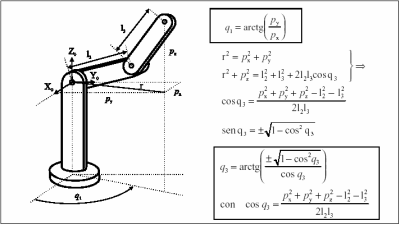
\includegraphics[scale=1.2]{imagenes/cinematica.png} imagen 1.2
\end{center}
\begin{large}
Es adecuado para robots de pocos grados de libertad o para el caso de que se consideren solo los primeros grados de libertad para posicionar el extremo.

El procedimiento se basa en encontrar un número suficiente de relaciones geométricas en las que intervendrán las coordenadas del extremo del robot, sus coordenadas articulares y las dimensiones físicas de sus elementos.
\end{large}
\begin{center}
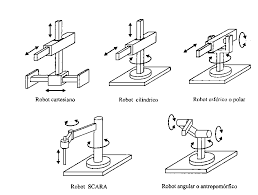
\includegraphics[scale=1.2]{imagenes/recta.png} imagen 1.3
\end{center}

 \begin{huge}
\textbf{Referencias}
\end{huge}
\begin{normalsize}
@article{mozo2017mecanismos,
  title={Mecanismos articulados: Geometr{\'\i}a Din{\'a}mica y Cinem{\'a}tica en un entorno educativo STEM},
  author={Mozo, Francisco Javier Manzano and Garc{\'\i}a, Melchor G{\'o}mez and Mozo-Fern{\'a}ndez, Jorge},
  journal={Innoeduca: international journal of technology and educational innovation},
  volume={3},
  number={1},
  pages={15--27},
  year={2017},
  publisher={Grupo de Investigaci{\'o}n Innoeduca}
}
\end{normalsize}
\end{document}